\makesection{Benchmarking}

\begin{frame}{Dataset - LFM\_1b\_artist}
\small
Il primo dataset utilizzato è LFM\_1b\_artist, un dataset di ascolti musicali contenente informazioni riguardanti le interazioni tra utenti e artisti musicali

\begin{table}[H]
\centering
\begin{tabular}{|c|c|}
\hline
\textbf{Feature} & \textbf{Valore} \\
\hline
Numero di utenti & 120322 \\
\hline
Numero di item & 3123496 \\
\hline
Numero di interazioni & 65133026 \\
\hline
Sparsità & 0.9998266933373666 \\
\hline
avg\_interactions & 541.3226675088513 \\
\hline
\end{tabular}
\caption{Statistiche dataset LFM\_1b\_artist}
\end{table}
\end{frame}

\begin{frame}{Dataset - LFM\_1b\_artist}
    Questo risultava essere troppo grande per le risorse a disposizione, quindi così processato:
    \begin{itemize}
        \item  \textbf{Filtraggio}: il dataset è stato filtrato eliminando tutte le interazioni in cui erano coinvolti utenti e/o item
        con meno di 5 interazioni
        \item  \textbf{Sampling}:sampling casuale di 50000 items e 20000 utenti. Sono sate mantenute solo le interazioni che coinvolgevano questi utenti e items
        \item \textbf{Stratificazione}: Sono state effettuate le seguenti stratificazioni per utente in modo da mantenere la distribuzione delle interazioni: 75\% , 50\%, 25\%
    \end{itemize}
\end{frame}




\begin{frame}{Dataset - MovieLens10M}
    \small
    E' un dataset di valutazioni di film, contenente informazioni riguardanti le valutazioni date dagli utenti ai film. In questo caso sono presenti 10 milioni di valutazioni. E' stato anche aggiunto un knowledge graph contenente informazioni riguardanti i film e gli attori.
    
    \begin{table}[H]
    \centering
    \begin{tabular}{|c|c|}
    \hline
    \textbf{Feature} & \textbf{Valore} \\
    \hline
    Numero di utenti & 69878 \\
    \hline
    Numero di item & 10677 \\
    \hline
    Numero di interazioni & 10000054 \\
    \hline
    Sparsità & 0.9865966722939162 \\
    \hline
    avg\_interactions & 143.10732991785684 \\
    \hline
    \end{tabular}
    \caption{Statistiche MovieLens10M}
    \end{table}
    \end{frame}
    
    \begin{frame}{Dataset - MovieLens10M}
        Anche questo risultava essere troppo grande per le risorse a disposizione, quindi così processato:
        \begin{itemize}
            \item  \textbf{Filtraggio}: il dataset è stato filtrato eliminando tutte le interazioni in cui erano coinvolti utenti e/o item
            con meno di 5 interazioni
            \item  \textbf{Sampling}:sampling casuale di 50000 utenti e 10000 items. Sono sate mantenute solo le interazioni che coinvolgevano questi utenti e items
        \end{itemize}
    \end{frame}


\begin{frame}{Emissioni - LFM\_1b\_artist}
        \begin{wrapfigure}{r}{0.45\textwidth}
        \centering
        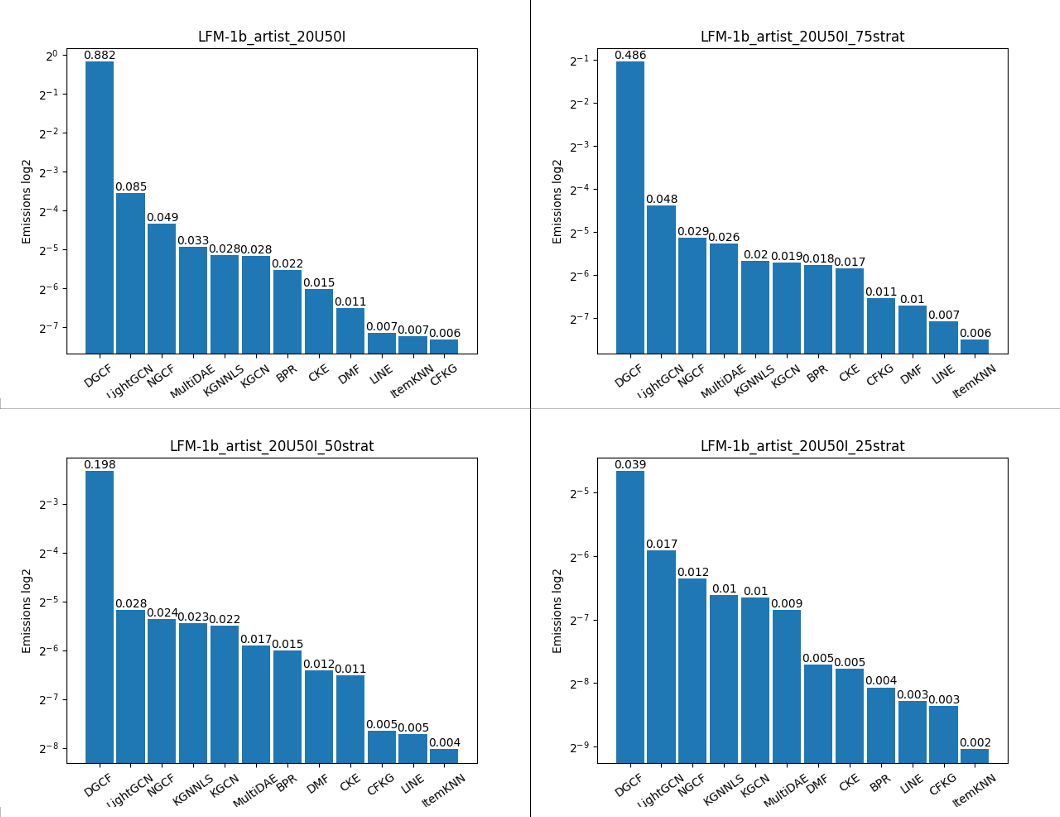
\includegraphics[width=0.45\textwidth]{images/EmissioniLFM.png}
        \caption{Emissioni LFM\_1b\_artist}
    \end{wrapfigure}
    \small
    Si può subito notare come DGCF è il modello che emette più CO2 in assoluto, da 2 a 10 volte di più rispetto agli altri modelli a seconda del dataset.
    LightGCN e NCFG sono rispettivamente il secondo e il terzo modello che emettono più CO2.
    Questi due modelli sono di tipo general, ma nonostante ciò emettono di più rispetto ad altri di tipo knowledge-aware, come per esempio il KGCN
\end{frame}

\begin{frame}{Emissioni - MovieLens10M}
    \begin{wrapfigure}{r}{0.45\textwidth}
    \centering
    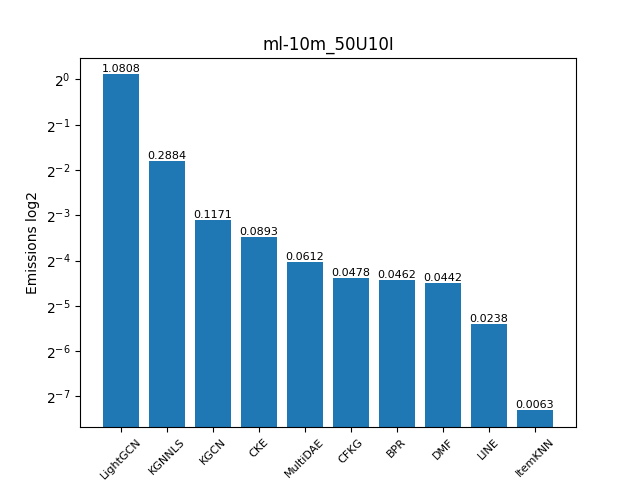
\includegraphics[width=0.45\textwidth]{images/emissions_ml-10m_50U10I.png}
    \caption{Emissioni MovieLens10M}
\end{wrapfigure}
\small
E' possibile notare come molti modelli rispetto al dataset LFM-1b\_artist\_20U50I abbiano emissioni di CO2 molto più alte (a volte anche 10 volte tanto).
Ciò sicuramente è dovuto al fatto che il numero delle interazioni presenti in questo dataset sono circa 10 volte quelle del dataset LFM-1b\_artist\_20U50I.
E' possibile comunque notare come i modelli che le emissioni dei modelli seguono circa lo stesso ordine dei dataset precedenti, confermando le tendenze.
\end{frame}


\begin{frame}{Trade - Off}
    \begin{wrapfigure}{r}{0.45\textwidth}
    \centering
    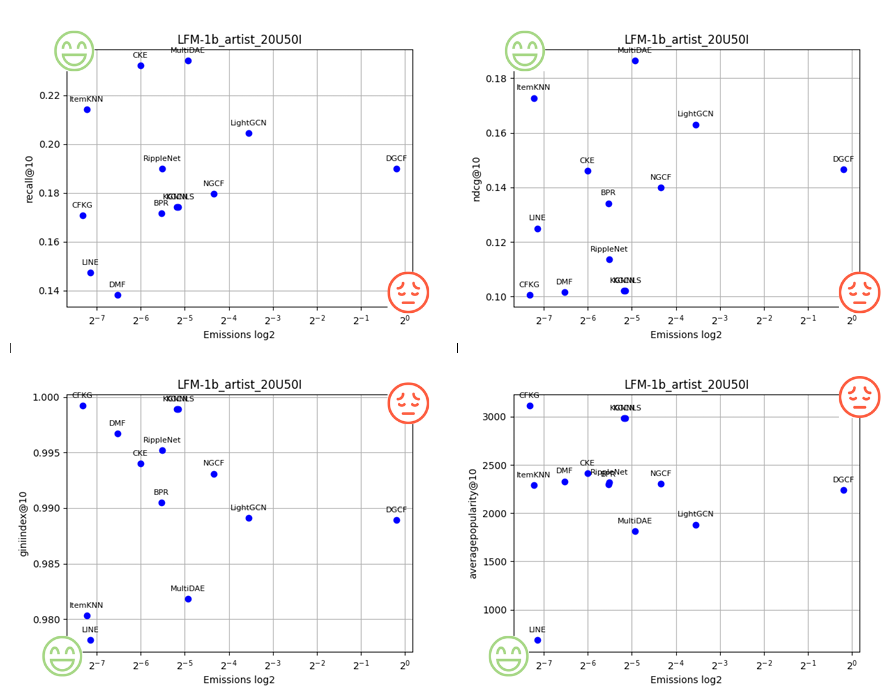
\includegraphics[width=0.45\textwidth]{images/TradeOff.png}
    \caption{Trade-Off}
\end{wrapfigure}

Per ogni dataset sono stati creati grafici che mostrano il trade-off tra emissioni e performance simili a quello mostrato in figura. In generale DGCF è il modello in cui il trade-off mostra i risultati peggiori. In genere ItemKNN risulta essere il migliore nel trade-off per le metriche di ranking mentre LINE il migliore per le metriche di popolarità e giniindex.
\end{frame}




\begin{frame}{Regressore - Dataset Completo}
    \begin{wrapfigure}{r}{0.5\textwidth}
    \centering
    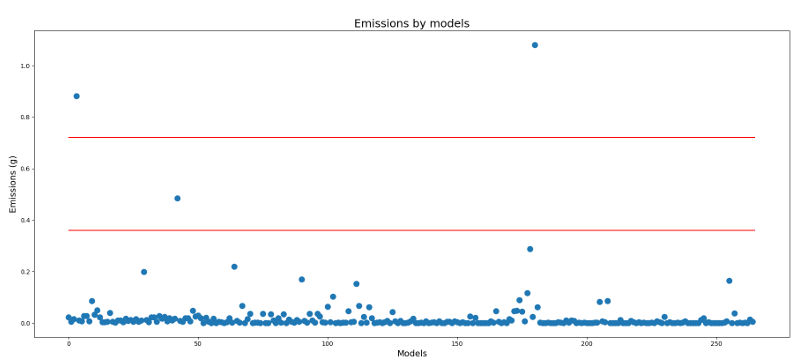
\includegraphics[width=0.5\textwidth]{images/distribuzioneCompleta.png}
    \caption{Nuova distribuzione dei dati}
\end{wrapfigure}

Come è possibile notare i nuovi esperimenti hanno portato a un'ulteriore sbilanciamento nel dataset, in quanto tutti gli esperimenti con DGCF e altri modelli svettano sui risultati degli altri modelli in emissioni.
Questo si riflette nei risultati ottenuti dai modelli di regressione. Per quanto riguarda i modelli,
sono stati eseguti addestramenti con diversi split tra training e test set.

\end{frame}


\begin{frame}{Regressore - Analisi dei risultati Dataset Completo}
    \begin{wrapfigure}{r}{0.5\textwidth}
    \centering
    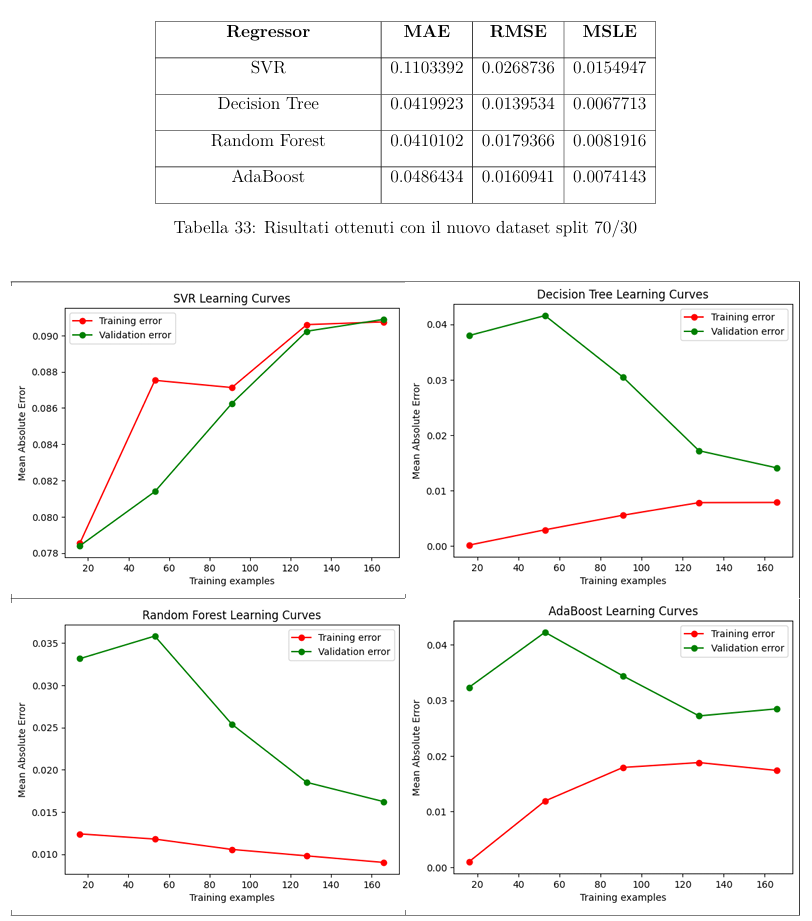
\includegraphics[width=0.3\textwidth]{images/RisultatiRegCompleto.png}
    \caption{Risultati con dataset completo}
\end{wrapfigure}
\small
Sono stati eseguti addestramenti con i seguenti split:
\begin{itemize}
    \item 50\% training, 50\% test
    \item 60\% training, 40\% test
    \item 70\% training, 30\% test
    \item 80\% training, 20\% test
    \item 90\% training, 10\% test
\end{itemize} 
I migliori risultati sono stati ottenuti con lo split 70-30, con il Decision Tree Regressor che risulta essere il modello migliore.
\end{frame}



\begin{frame}{Regressore - Dataset Azure}
    \begin{wrapfigure}{r}{0.5\textwidth}
    \centering
    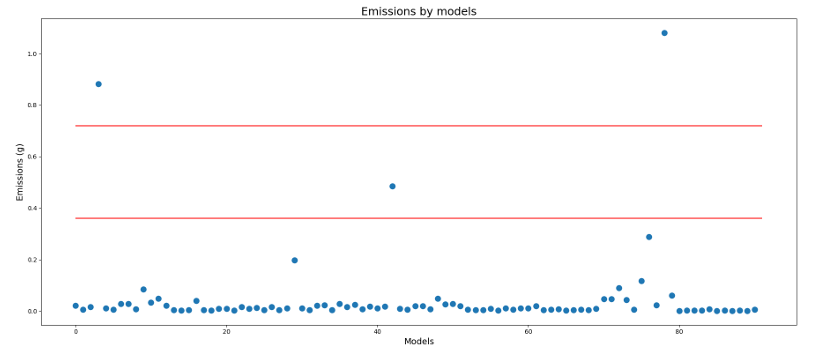
\includegraphics[width=0.5\textwidth]{images/distribuzioneAzure.png}
    \caption{Nuova distribuzione dei dati}
\end{wrapfigure}

E' stato creato un nuovo dataset con i risultati ottenuti solo sugli esperimenti eseguiti su Azure per avere un regressore specifico per gli esperimenti eseguiti su tale macchina.

\end{frame}


\begin{frame}{Regressore - Analisi dei risultati Dataset Azure}
    \begin{wrapfigure}{r}{0.5\textwidth}
    \centering
    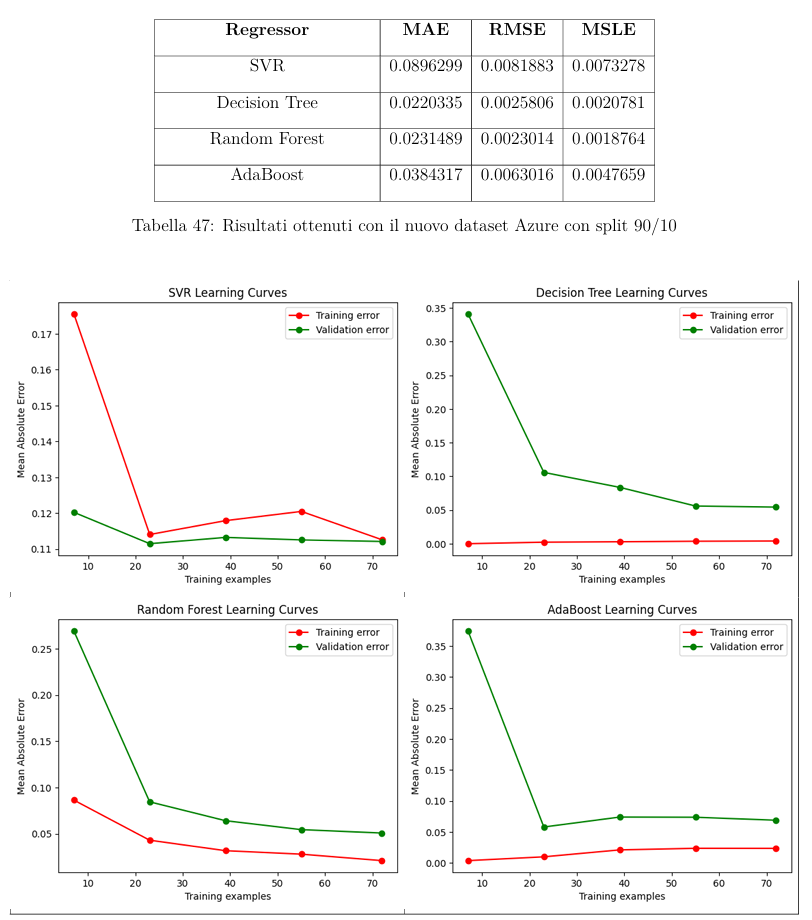
\includegraphics[width=0.3\textwidth]{images/RisultatiRegAzure.png}
    \caption{Risultati con dataset completo}
\end{wrapfigure}
\small
Sono stati eseguti addestramenti con i seguenti split:
\begin{itemize}
    \item 50\% training, 50\% test
    \item 60\% training, 40\% test
    \item 70\% training, 30\% test
    \item 80\% training, 20\% test
    \item 90\% training, 10\% test
\end{itemize} 
I migliori risultati sono stati ottenuti con lo split 90-10, con il Decision Tree Regressor che risulta essere il modello migliore.
\end{frame}


\begin{frame}{Errori nelle classi}
Il dataset è stato diviso in 3 classi, ovvero \textbf{low}, \textbf{medium} e \textbf{high}, in base ai valori di emissioni di CO2 (rispettivamente codificate con 0,1,2).
Per ogni elemento del test set, sono stati calcolati gli errori e successivamente si è proceduto a calcolare la media degli errori per ogni classe.
Gli errori sono stati calcolati come segue:
\begin{itemize}
    \item \textbf{Errore assoluto}:\begin{equation*}
        |y - \hat{y}|
         \end{equation*}
    \item \textbf{Errore percentuale}: \begin{equation*}
        \frac{|y - \hat{y}|}{y} \cdot 100
    \end{equation*}
\end{itemize}
dove $y$ è il valore reale e $\hat{y}$ è il valore predetto.
\end{frame}

\begin{frame}{Errori nelle classi}
\scriptsize 
\textbf{Dataset Completo}
\begin{itemize}
    \item \textbf{low\_bound}:0.36027045739563296
    \item \textbf{high\_bound}: 0.7205403996360675.
\end{itemize}


\begin{table}[H]
    \centering
    \begin{tabular}{|c|c|c|c|}
        \hline
        \textbf{Classe} &  \textbf{Numero elementi} & \textbf{Errore assoluto medio} & \textbf{Errore percentuale medio} \\ \hline
        low             & 78                & 0.021805                   & 813            \\ \hline
        medium          & 0                & -                  & -            \\ \hline
        high            & 2                & 0.790026                   & 80            \\ \hline
    \end{tabular}
    \caption{Errori delle classi per il dataset completo}
\end{table}



\textbf{Dataset Azure}
\begin{itemize}
    \item \textbf{low\_bound}: 0.3610033427811713
    \item  \textbf{high\_bound}: 0.7203571782896829.
\end{itemize}

\begin{table}[H]
    \centering
    \begin{tabular}{|c|c|c|c|}
        \hline
        \textbf{Classe} &  \textbf{Numero elementi} & \textbf{Errore assoluto medio} & \textbf{Errore percentuale medio} \\ \hline
        low             & 78                & 0.044774                   & 188.63            \\ \hline
        medium          & 0                & -                  & -            \\ \hline
        high            & 2                & 0.588654                   & 66.76            \\ \hline
    \end{tabular}
    \caption{Errori delle classi per il dataset Azure}
\end{table}

\end{frame}